\documentclass[11pt, letterpaper]{article}

% Fonts and Encoding
\usepackage[utf8]{inputenc}
\usepackage[T1]{fontenc}
\usepackage{lmodern} % High-quality Latin Modern vector font

% Math and Symbols
\usepackage{amsmath, amssymb, amsthm, amsfonts, mathrsfs, mathtools}

% Layout and Geometry
\usepackage{geometry}
\geometry{letterpaper, margin=1in}
\setlength{\parindent}{0pt}
\setlength{\parskip}{0.6em}

% Formatting and Graphics
\usepackage{graphicx, xcolor, enumitem, booktabs, array, tabularx}

% TikZ for Illustrations
\usepackage{tikz}
\usetikzlibrary{arrows.meta, positioning, shapes.geometric, calc, backgrounds, matrix}

% Clickable Links and TOC
\usepackage{hyperref}
\hypersetup{
    colorlinks=true,
    linkcolor=blue,
    filecolor=magenta,      
    urlcolor=cyan,
    pdftitle={Advanced Mathematics Topic},
}

% Theorem Environments
\newtheorem{theorem}{Theorem}[section]
\newtheorem{lemma}[theorem]{Lemma}
\newtheorem{proposition}[theorem]{Proposition}
\newtheorem{corollary}[theorem]{Corollary}
\theoremstyle{definition}
\newtheorem{definition}{Definition}[section]
\newtheorem{axiom}{Axiom}[section]
\newtheorem{example}{Example}[section]
\theoremstyle{remark}
\newtheorem{remark}{Remark}[section]

% Custom Commands (Enforced standard notation)
\newcommand{\R}{\mathbb{R}}
\newcommand{\N}{\mathbb{N}}
\newcommand{\Z}{\mathbb{Z}}
\newcommand{\Q}{\mathbb{Q}}
\newcommand{\E}{\mathbb{E}}
\newcommand{\Prob}{\mathbb{P}}
\newcommand{\F}{\mathcal{F}}

\begin{document}

\title{\textbf{Transforms of Periodic and Power Functions}}
\author{Tashfeen Omran}
\date{\today}
\maketitle

\tableofcontents
\newpage

\section{Part 1: Comprehensive Introduction, Context, and Prerequisites}

\subsection{Core Concepts}
The Laplace transform is a powerful integral transform used to switch a function from the time domain ($t$) to the complex frequency domain ($s$). In this chapter, we extend the Laplace transform to two special classes of functions: \textbf{Periodic Functions} and \textbf{Power Functions} (specifically those with non-integer exponents).

A function $f(t)$ is \textbf{periodic} with period $T > 0$ if $f(t + T) = f(t)$ for all $t$ in the domain of $f$. Common examples include sine, cosine, square waves, and sawtooth waves. Because these functions repeat infinitely, computing their Laplace transform over the interval $[0, \infty)$ can be simplified by evaluating the integral over just a single period $[0, T]$ and applying a geometric series summation.

To handle non-integer power functions like $f(t) = t^{1/2}$, we introduce the \textbf{Gamma Function}, $\Gamma(r)$, which serves as a continuous extension of the factorial function.

\subsection{Intuition and Derivation}
\textbf{Periodic Functions:} 
Consider the definition of the Laplace transform for a periodic function $f(t)$ with period $T$:
\[ \mathcal{L}\{f\}(s) = \int_0^\infty e^{-st} f(t) \, dt \]
We can split this infinite integral into a sum of integrals over each period:
\[ \mathcal{L}\{f\}(s) = \sum_{n=0}^\infty \int_{nT}^{(n+1)T} e^{-st} f(t) \, dt \]
By making the substitution $u = t - nT$, and using the periodic property $f(u + nT) = f(u)$, the integral becomes:
\[ \mathcal{L}\{f\}(s) = \sum_{n=0}^\infty e^{-nsT} \int_0^T e^{-su} f(u) \, du \]
The sum $\sum_{n=0}^\infty (e^{-sT})^n$ is a geometric series that converges to $\frac{1}{1 - e^{-sT}}$ for $s > 0$. Thus, the transform of the entire infinite periodic function is simply the transform of its first period (the "windowed" version) divided by $1 - e^{-sT}$.

\textbf{The Gamma Function:}
For an integer $n$, $\mathcal{L}\{t^n\} = \frac{n!}{s^{n+1}}$. To generalize this to $t^r$ where $r$ is a real number, we need a way to compute $r!$. The Gamma function is defined as $\Gamma(r) = \int_0^\infty e^{-u} u^{r-1} \, du$. Using integration by parts, one can show that $\Gamma(r+1) = r\Gamma(r)$, which perfectly mirrors the factorial property $(n+1)! = (n+1)n!$.

\subsection{Historical Context and Motivation}
The Laplace transform was formalized by Pierre-Simon Laplace in the late 18th century, building on earlier work by Leonhard Euler. The motivation was to transform complex differential equations into simpler algebraic equations. Periodic functions are ubiquitous in physics and engineering—representing AC circuits, mechanical vibrations, and signal processing. The ability to easily transform periodic functions without integrating to infinity was a monumental leap for electrical engineers analyzing continuous wave signals. The Gamma function was introduced by Euler in the 1720s specifically to solve the problem of interpolating the factorial function for non-integer values.

\subsection{Key Formulas}
\begin{itemize}
    \item \textbf{Transform of a Periodic Function:} If $f(t)$ has period $T$, then
    \[ \mathcal{L}\{f\}(s) = \frac{\int_0^T e^{-st} f(t) \, dt}{1 - e^{-sT}} = \frac{F_T(s)}{1 - e^{-sT}} \]
    where $F_T(s)$ is the transform of the windowed function $f_T(t) = f(t)[u(t) - u(t-T)]$.
    \item \textbf{Gamma Function:} $\Gamma(r) = \int_0^\infty e^{-u} u^{r-1} \, du$ for $r > 0$.
    \item \textbf{Gamma Recursive Relation:} $\Gamma(r+1) = r\Gamma(r)$.
    \item \textbf{Transform of a Power Function:} $\mathcal{L}\{t^r\}(s) = \frac{\Gamma(r+1)}{s^{r+1}}$ for $r > -1$.
\end{itemize}

\subsection{Prerequisites}
To succeed in this topic, you must be proficient in:
1. \textbf{Integration by Parts:} Essential for evaluating $\int_0^T e^{-st} t \, dt$.
2. \textbf{Geometric Series:} Understanding $\sum_{n=0}^\infty x^n = \frac{1}{1-x}$ for $|x| < 1$.
3. \textbf{Taylor/Maclaurin Series:} Required for expanding functions like $\sin(t)$ or $e^{-1/s}$ to compute transforms term-by-term.
4. \textbf{Basic Laplace Transforms:} Knowing the transforms of $e^{at}$, $\sin(bt)$, $\cos(bt)$, and the translation theorems.

\newpage
\section{Part 2: Detailed Homework Solutions}

\textbf{Problem 1:} Determine $\mathcal{L}\{f\}$, where $f(t) = t$ for $0 < t < 2$, and $f(t)$ has period $2$. Also graph $f(t)$.

\textbf{Solution:}
First, we identify the period $T = 2$. The formula for the Laplace transform of a periodic function is:
\[ \mathcal{L}\{f\}(s) = \frac{1}{1 - e^{-2s}} \int_0^2 e^{-st} t \, dt \]
We evaluate the integral using integration by parts. Let $u = t$ and $dv = e^{-st} \, dt$. Then $du = dt$ and $v = -\frac{1}{s}e^{-st}$.
\begin{align*}
    \int_0^2 t e^{-st} \, dt &= \left[ -\frac{t}{s}e^{-st} \right]_0^2 - \int_0^2 \left(-\frac{1}{s}e^{-st}\right) \, dt \\
    &= \left( -\frac{2}{s}e^{-2s} - 0 \right) - \left[ \frac{1}{s^2}e^{-st} \right]_0^2 \\
    &= -\frac{2}{s}e^{-2s} - \left( \frac{1}{s^2}e^{-2s} - \frac{1}{s^2} \right) \\
    &= \frac{1}{s^2} - e^{-2s} \left( \frac{2}{s} + \frac{1}{s^2} \right)
\end{align*}
Substituting this back into the periodic transform formula:
\[ \mathcal{L}\{f\}(s) = \frac{\frac{1}{s^2} - e^{-2s} \left( \frac{2}{s} + \frac{1}{s^2} \right)}{1 - e^{-2s}} = \frac{1 - e^{-2s}(2s + 1)}{s^2(1 - e^{-2s})} \]

\begin{center}
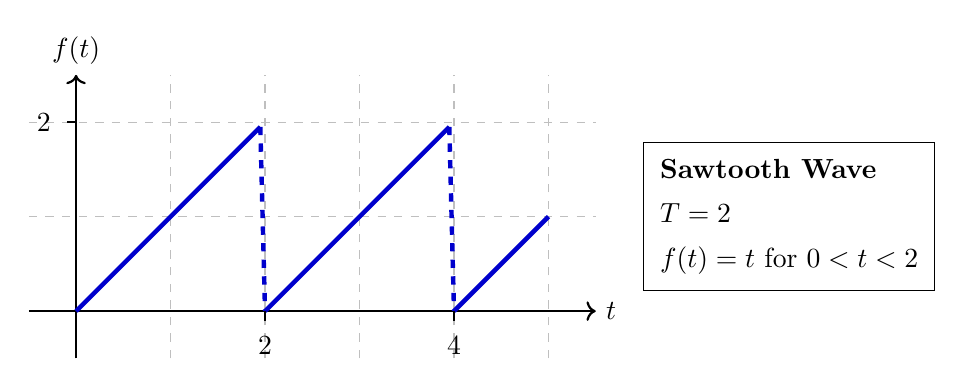
\begin{tikzpicture}[scale=1.2]
    \fill[white] (-0.5, -0.5) rectangle (5.5, 2.5);
    \draw[lightgray, thin, dashed] (-0.5, -0.5) grid (5.5, 2.5);
    \draw[->, thick] (-0.5, 0) -- (5.5, 0) node[right] {$t$};
    \draw[->, thick] (0, -0.5) -- (0, 2.5) node[above] {$f(t)$};
    
    \draw[ultra thick, blue!80!black] (0,0) -- (1.95,1.95);
    \draw[ultra thick, blue!80!black, dashed] (1.95,1.95) -- (2,0);
    \draw[ultra thick, blue!80!black] (2,0) -- (3.95,1.95);
    \draw[ultra thick, blue!80!black, dashed] (3.95,1.95) -- (4,0);
    \draw[ultra thick, blue!80!black] (4,0) -- (5,1);
    
    \draw[thick] (2,0) -- (2,-0.1) node[below=2pt] {$2$};
    \draw[thick] (4,0) -- (4,-0.1) node[below=2pt] {$4$};
    \draw[thick] (0,2) -- (-0.1,2) node[left=2pt] {$2$};
    
    \node[align=left, anchor=west, fill=white, draw=black, inner sep=6pt] at (6, 1) {
        \textbf{Sawtooth Wave} \\[4pt]
        $T = 2$ \\[4pt]
        $f(t) = t$ for $0 < t < 2$
    };
\end{tikzpicture}
\end{center}

\vspace{1em}
\textbf{Problem 2:} Determine $\mathcal{L}\{f\}$, where $f(t) = e^t$ for $0 < t < 1$, and $f(t)$ has period $1$.

\textbf{Solution:}
The period is $T = 1$. The Laplace transform is:
\[ \mathcal{L}\{f\}(s) = \frac{1}{1 - e^{-s}} \int_0^1 e^{-st} e^t \, dt = \frac{1}{1 - e^{-s}} \int_0^1 e^{(1-s)t} \, dt \]
Evaluating the integral:
\begin{align*}
    \int_0^1 e^{(1-s)t} \, dt &= \left[ \frac{1}{1-s} e^{(1-s)t} \right]_0^1 \\
    &= \frac{1}{1-s} \left( e^{1-s} - 1 \right)
\end{align*}
Thus, the Laplace transform is:
\[ \mathcal{L}\{f\}(s) = \frac{e^{1-s} - 1}{(1-s)(1 - e^{-s})} \]

\vspace{1em}
\textbf{Problem 3:} Determine $\mathcal{L}\{f\}$, where $f(t) = e^{-t}$ for $0 < t < 1$, $f(t) = 1$ for $1 < t < 2$, and $f(t)$ has period $2$.

\textbf{Solution:}
The period is $T = 2$. We split the integral over the two sub-intervals:
\[ \mathcal{L}\{f\}(s) = \frac{1}{1 - e^{-2s}} \left( \int_0^1 e^{-st} e^{-t} \, dt + \int_1^2 e^{-st} (1) \, dt \right) \]
Evaluate the first integral:
\[ \int_0^1 e^{-(s+1)t} \, dt = \left[ -\frac{1}{s+1} e^{-(s+1)t} \right]_0^1 = \frac{1 - e^{-(s+1)}}{s+1} \]
Evaluate the second integral:
\[ \int_1^2 e^{-st} \, dt = \left[ -\frac{1}{s} e^{-st} \right]_1^2 = \frac{e^{-s} - e^{-2s}}{s} \]
Combining these gives the final transform:
\[ \mathcal{L}\{f\}(s) = \frac{1}{1 - e^{-2s}} \left( \frac{1 - e^{-(s+1)}}{s+1} + \frac{e^{-s} - e^{-2s}}{s} \right) \]

\vspace{1em}
\textbf{Problem 4:} Determine $\mathcal{L}\{f\}$, where $f(t) = t$ for $0 < t < 1$, $f(t) = 1-t$ for $1 < t < 2$, and $f(t)$ has period $2$.

\textbf{Solution:}
The period is $T = 2$. We split the integral:
\[ \mathcal{L}\{f\}(s) = \frac{1}{1 - e^{-2s}} \left( \int_0^1 t e^{-st} \, dt + \int_1^2 (1-t) e^{-st} \, dt \right) \]
From Problem 1, we know the antiderivative of $t e^{-st}$ is $-\frac{t}{s}e^{-st} - \frac{1}{s^2}e^{-st}$.
First integral:
\[ \int_0^1 t e^{-st} \, dt = \left[ -\frac{t}{s}e^{-st} - \frac{1}{s^2}e^{-st} \right]_0^1 = -\frac{1}{s}e^{-s} - \frac{1}{s^2}e^{-s} + \frac{1}{s^2} \]
Second integral:
\begin{align*}
    \int_1^2 (1-t) e^{-st} \, dt &= \int_1^2 e^{-st} \, dt - \int_1^2 t e^{-st} \, dt \\
    &= \left[ -\frac{1}{s}e^{-st} \right]_1^2 - \left[ -\frac{t}{s}e^{-st} - \frac{1}{s^2}e^{-st} \right]_1^2 \\
    &= \left( -\frac{1}{s}e^{-2s} + \frac{1}{s}e^{-s} \right) - \left( -\frac{2}{s}e^{-2s} - \frac{1}{s^2}e^{-2s} + \frac{1}{s}e^{-s} + \frac{1}{s^2}e^{-s} \right) \\
    &= \frac{1}{s}e^{-2s} + \frac{1}{s^2}e^{-2s} - \frac{1}{s^2}e^{-s}
\end{align*}
Adding the two integrals together:
\[ \left( \frac{1}{s^2} - \frac{1}{s}e^{-s} - \frac{1}{s^2}e^{-s} \right) + \left( \frac{1}{s}e^{-2s} + \frac{1}{s^2}e^{-2s} - \frac{1}{s^2}e^{-s} \right) = \frac{1}{s^2} - \frac{1}{s}e^{-s} - \frac{2}{s^2}e^{-s} + \frac{1}{s}e^{-2s} + \frac{1}{s^2}e^{-2s} \]
Thus:
\[ \mathcal{L}\{f\}(s) = \frac{1 - s e^{-s} - 2e^{-s} + s e^{-2s} + e^{-2s}}{s^2(1 - e^{-2s})} \]

\vspace{1em}
\textbf{Problem 5:} Determine $\mathcal{L}\{f\}$, where the periodic function is described by its graph (Square wave, $f(t)=1$ for $0<t<a$, $f(t)=0$ for $a<t<2a$, period $2a$).

\textbf{Solution:}
The period is $T = 2a$. The function is $f(t) = 1$ on $(0, a)$ and $0$ on $(a, 2a)$.
\[ \mathcal{L}\{f\}(s) = \frac{1}{1 - e^{-2as}} \int_0^a 1 \cdot e^{-st} \, dt \]
Evaluating the integral:
\[ \int_0^a e^{-st} \, dt = \left[ -\frac{1}{s} e^{-st} \right]_0^a = \frac{1 - e^{-as}}{s} \]
Substitute this into the formula:
\[ \mathcal{L}\{f\}(s) = \frac{1 - e^{-as}}{s(1 - e^{-2as})} \]
Notice that $1 - e^{-2as}$ is a difference of squares: $(1 - e^{-as})(1 + e^{-as})$. Canceling the common term yields:
\[ \mathcal{L}\{f\}(s) = \frac{1}{s(1 + e^{-as})} \]

\vspace{1em}
\textbf{Problem 6:} Determine $\mathcal{L}\{f\}$, where the periodic function is described by its graph (Sawtooth wave, $f(t) = t/a$ for $0 < t < a$, period $a$).

\textbf{Solution:}
The period is $T = a$. The function is $f(t) = \frac{t}{a}$ on $(0, a)$.
\[ \mathcal{L}\{f\}(s) = \frac{1}{1 - e^{-as}} \int_0^a \frac{t}{a} e^{-st} \, dt \]
Using integration by parts (as in Problem 1):
\begin{align*}
    \frac{1}{a} \int_0^a t e^{-st} \, dt &= \frac{1}{a} \left[ -\frac{t}{s}e^{-st} - \frac{1}{s^2}e^{-st} \right]_0^a \\
    &= \frac{1}{a} \left( -\frac{a}{s}e^{-as} - \frac{1}{s^2}e^{-as} + \frac{1}{s^2} \right) \\
    &= \frac{1 - e^{-as} - as e^{-as}}{a s^2}
\end{align*}
Thus, the transform is:
\[ \mathcal{L}\{f\}(s) = \frac{1 - e^{-as} - as e^{-as}}{a s^2 (1 - e^{-as})} \]

\vspace{1em}
\textbf{Problem 7:} Determine $\mathcal{L}\{f\}$, where the periodic function is described by its graph (Triangular wave, $f(t) = t/a$ for $0 < t < a$, $f(t) = 2 - t/a$ for $a < t < 2a$, period $2a$).

\textbf{Solution:}
The period is $T = 2a$.
\[ \mathcal{L}\{f\}(s) = \frac{1}{1 - e^{-2as}} \left( \int_0^a \frac{t}{a} e^{-st} \, dt + \int_a^{2a} \left(2 - \frac{t}{a}\right) e^{-st} \, dt \right) \]
From Problem 6, the first integral is $\frac{1 - e^{-as} - as e^{-as}}{a s^2}$.
For the second integral, let $u = t - a$, so $t = u + a$ and $dt = du$. The limits change from $0$ to $a$.
\begin{align*}
    \int_a^{2a} \left(2 - \frac{t}{a}\right) e^{-st} \, dt &= \int_0^a \left(2 - \frac{u+a}{a}\right) e^{-s(u+a)} \, du \\
    &= e^{-as} \int_0^a \left(1 - \frac{u}{a}\right) e^{-su} \, du \\
    &= e^{-as} \left( \int_0^a e^{-su} \, du - \frac{1}{a} \int_0^a u e^{-su} \, du \right) \\
    &= e^{-as} \left( \frac{1 - e^{-as}}{s} - \frac{1 - e^{-as} - as e^{-as}}{a s^2} \right) \\
    &= e^{-as} \left( \frac{as - as e^{-as} - 1 + e^{-as} + as e^{-as}}{a s^2} \right) \\
    &= \frac{as e^{-as} - e^{-as} + e^{-2as}}{a s^2}
\end{align*}
Adding the two integrals:
\[ \frac{1 - e^{-as} - as e^{-as} + as e^{-as} - e^{-as} + e^{-2as}}{a s^2} = \frac{1 - 2e^{-as} + e^{-2as}}{a s^2} = \frac{(1 - e^{-as})^2}{a s^2} \]
Now, divide by $1 - e^{-2as} = (1 - e^{-as})(1 + e^{-as})$:
\[ \mathcal{L}\{f\}(s) = \frac{(1 - e^{-as})^2}{a s^2 (1 - e^{-as})(1 + e^{-as})} = \frac{1 - e^{-as}}{a s^2 (1 + e^{-as})} \]
This can also be written using hyperbolic tangent as $\frac{1}{a s^2} \tanh\left(\frac{as}{2}\right)$.

\vspace{1em}
\textbf{Problem 8:} Determine $\mathcal{L}\{f\}$, where the periodic function is described by its graph (Half-rectified sine wave, $f(t) = \sin t$ for $0 < t < \pi$, $f(t) = 0$ for $\pi < t < 2\pi$, period $2\pi$).

\textbf{Solution:}
The period is $T = 2\pi$.
\[ \mathcal{L}\{f\}(s) = \frac{1}{1 - e^{-2\pi s}} \int_0^\pi \sin(t) e^{-st} \, dt \]
We use the standard integration formula $\int e^{at} \sin(bt) \, dt = \frac{e^{at}}{a^2+b^2}(a \sin(bt) - b \cos(bt))$. Here $a = -s$ and $b = 1$.
\begin{align*}
    \int_0^\pi e^{-st} \sin(t) \, dt &= \left[ \frac{e^{-st}}{s^2 + 1} (-s \sin(t) - \cos(t)) \right]_0^\pi \\
    &= \frac{e^{-\pi s}}{s^2 + 1} (0 - (-1)) - \frac{1}{s^2 + 1} (0 - 1) \\
    &= \frac{e^{-\pi s} + 1}{s^2 + 1}
\end{align*}
Substitute this into the transform formula:
\[ \mathcal{L}\{f\}(s) = \frac{1 + e^{-\pi s}}{(s^2 + 1)(1 - e^{-2\pi s})} \]
Since $1 - e^{-2\pi s} = (1 - e^{-\pi s})(1 + e^{-\pi s})$, we can cancel the common factor:
\[ \mathcal{L}\{f\}(s) = \frac{1}{(s^2 + 1)(1 - e^{-\pi s})} \]

\vspace{1em}
\textbf{Problem 9:} Show that if $\mathcal{L}\{g\}(s) = [(s+\alpha)(1-e^{-Ts})]^{-1}$, where $T > 0$ is fixed, then
\[ g(t) = e^{-\alpha t} + e^{-\alpha(t-T)}u(t-T) + e^{-\alpha(t-2T)}u(t-2T) + \dots \]

\textbf{Solution:}
We are given $\mathcal{L}\{g\}(s) = \frac{1}{s+\alpha} \cdot \frac{1}{1-e^{-Ts}}$.
Using the geometric series expansion $\frac{1}{1-x} = 1 + x + x^2 + \dots$ for $|x| < 1$, we let $x = e^{-Ts}$:
\[ \frac{1}{1-e^{-Ts}} = 1 + e^{-Ts} + e^{-2Ts} + e^{-3Ts} + \dots = \sum_{n=0}^\infty e^{-nTs} \]
Multiply this series by $\frac{1}{s+\alpha}$:
\[ \mathcal{L}\{g\}(s) = \sum_{n=0}^\infty \frac{e^{-nTs}}{s+\alpha} \]
We know that $\mathcal{L}^{-1}\left\{ \frac{1}{s+\alpha} \right\} = e^{-\alpha t}$.
By the Second Translation Theorem, $\mathcal{L}^{-1}\{ e^{-as} F(s) \} = f(t-a)u(t-a)$. Applying this to each term in the series with $a = nT$:
\[ \mathcal{L}^{-1}\left\{ \frac{e^{-nTs}}{s+\alpha} \right\} = e^{-\alpha(t-nT)} u(t-nT) \]
Summing these inverse transforms yields:
\[ g(t) = \sum_{n=0}^\infty e^{-\alpha(t-nT)} u(t-nT) = e^{-\alpha t} + e^{-\alpha(t-T)}u(t-T) + e^{-\alpha(t-2T)}u(t-2T) + \dots \]

\vspace{1em}
\textbf{Problem 10:} The function $g(t)$ in (9) can be expressed in a more convenient form.
(a) Show that for each $n = 0, 1, 2, \dots$, $g(t) = e^{-\alpha t} \left[ \frac{e^{(n+1)\alpha T} - 1}{e^{\alpha T} - 1} \right]$ for $nT < t < (n+1)T$.
(b) Let $v = t - (n+1)T$. Show that when $nT < t < (n+1)T$, then $-T < v < 0$ and $g(t) = \frac{e^{-\alpha v}}{e^{\alpha T} - 1} - \frac{e^{-\alpha t}}{e^{\alpha T} - 1}$.
(c) Sketch the graph of $g(t)$ for $\alpha = 1$ and $T = 2$.

\textbf{Solution:}
\textbf{(a)} For $t$ in the interval $nT < t < (n+1)T$, the step functions $u(t-kT)$ are $1$ for $k \le n$ and $0$ for $k > n$. Thus, the infinite series truncates to a finite sum:
\[ g(t) = \sum_{k=0}^n e^{-\alpha(t-kT)} = e^{-\alpha t} \sum_{k=0}^n e^{\alpha kT} = e^{-\alpha t} \sum_{k=0}^n (e^{\alpha T})^k \]
This is a finite geometric series with ratio $r = e^{\alpha T}$. Using the sum formula $\sum_{k=0}^n r^k = \frac{r^{n+1} - 1}{r - 1}$:
\[ g(t) = e^{-\alpha t} \left[ \frac{e^{(n+1)\alpha T} - 1}{e^{\alpha T} - 1} \right] \]

\textbf{(b)} Let $v = t - (n+1)T$. Since $nT < t < (n+1)T$, subtracting $(n+1)T$ gives $-T < v < 0$.
Substitute $(n+1)T = t - v$ into the expression from part (a):
\begin{align*}
    g(t) &= \frac{e^{-\alpha t} e^{\alpha(t-v)} - e^{-\alpha t}}{e^{\alpha T} - 1} \\
    &= \frac{e^{-\alpha v} - e^{-\alpha t}}{e^{\alpha T} - 1}
\end{align*}

\textbf{(c)} For $\alpha = 1$ and $T = 2$, $g(t) = \frac{e^{-v}}{e^2 - 1} - \frac{e^{-t}}{e^2 - 1}$. The first term is periodic with period $2$, and the second term decays exponentially. The graph looks like a sequence of exponential decays that get shifted upward slightly each period, eventually settling into a purely periodic steady state.

\vspace{1em}
\textbf{Problem 11:} Show that if $\mathcal{L}\{g\}(s) = \beta[(s^2+\beta^2)(1-e^{-Ts})]^{-1}$, then
\[ g(t) = \sin(\beta t) + [\sin \beta(t-T)]u(t-T) + [\sin \beta(t-2T)]u(t-2T) + \dots \]

\textbf{Solution:}
Similar to Problem 9, we expand the denominator as a geometric series:
\[ \mathcal{L}\{g\}(s) = \frac{\beta}{s^2+\beta^2} \sum_{n=0}^\infty e^{-nTs} = \sum_{n=0}^\infty \frac{\beta e^{-nTs}}{s^2+\beta^2} \]
We know that $\mathcal{L}^{-1}\left\{ \frac{\beta}{s^2+\beta^2} \right\} = \sin(\beta t)$.
Applying the Second Translation Theorem $\mathcal{L}^{-1}\{ e^{-as} F(s) \} = f(t-a)u(t-a)$ with $a = nT$:
\[ \mathcal{L}^{-1}\left\{ \frac{\beta e^{-nTs}}{s^2+\beta^2} \right\} = \sin(\beta(t-nT)) u(t-nT) \]
Summing these terms gives the desired result:
\[ g(t) = \sum_{n=0}^\infty \sin(\beta(t-nT)) u(t-nT) \]

\vspace{1em}
\textbf{Problem 12:} Use the result of Problem 11 to show that $\mathcal{L}^{-1}\left\{ \frac{1}{(s^2+1)(1-e^{-\pi s})} \right\}(t) = g(t)$, where $g(t)$ is the half-rectified sine wave.

\textbf{Solution:}
We apply the result of Problem 11 with $\beta = 1$ and $T = \pi$. The inverse transform is:
\[ g(t) = \sum_{n=0}^\infty \sin(t-n\pi) u(t-n\pi) \]
Using the trigonometric identity $\sin(t-n\pi) = \sin(t)\cos(n\pi) - \cos(t)\sin(n\pi) = (-1)^n \sin(t)$, we can write:
\[ g(t) = \sum_{n=0}^\infty (-1)^n \sin(t) u(t-n\pi) \]
Let's evaluate this sum on intervals of length $\pi$:
- For $0 < t < \pi$, only the $n=0$ term is active: $g(t) = \sin(t)$.
- For $\pi < t < 2\pi$, the $n=0$ and $n=1$ terms are active: $g(t) = \sin(t) - \sin(t) = 0$.
- For $2\pi < t < 3\pi$, the $n=0, 1, 2$ terms are active: $g(t) = \sin(t) - \sin(t) + \sin(t) = \sin(t)$.
This perfectly matches the definition of the half-rectified sine wave, which is $\sin(t)$ on $[0, \pi]$ and $0$ on $[\pi, 2\pi]$, repeating with period $2\pi$.

\vspace{1em}
\textbf{Problem 13:} Solve the initial value problem $y'' + 3y' + 2y = f(t); \quad y(0)=0, y'(0)=0$, where $f(t)$ is the periodic function from Problem 2 ($f(t)=e^t$ on $(0,1)$, period 1).

\textbf{Solution:}
Take the Laplace transform of both sides. Since initial conditions are zero, $\mathcal{L}\{y''\} = s^2 Y(s)$ and $\mathcal{L}\{y'\} = s Y(s)$.
\[ (s^2 + 3s + 2) Y(s) = F(s) \implies Y(s) = \frac{F(s)}{(s+1)(s+2)} \]
From Problem 2, $F(s) = \frac{e^{1-s}-1}{(1-s)(1-e^{-s})}$.
We can use partial fractions on the transfer function:
\[ \frac{1}{(s+1)(s+2)} = \frac{1}{s+1} - \frac{1}{s+2} \]
So, $Y(s) = F(s) \left( \frac{1}{s+1} - \frac{1}{s+2} \right)$.
Let $F_T(s) = \frac{e^{1-s}-1}{1-s}$ be the transform of the windowed function. Then:
\[ Y(s) = F_T(s) \left[ \frac{1}{(s+1)(1-e^{-s})} - \frac{1}{(s+2)(1-e^{-s})} \right] \]
By Problem 9, the inverse transform of $\frac{1}{(s+\alpha)(1-e^{-s})}$ is $h_\alpha(t) = \sum_{n=0}^\infty e^{-\alpha(t-n)} u(t-n)$.
Let $h(t) = h_1(t) - h_2(t)$. Then $y(t)$ is the convolution of the windowed function $f_T(t)$ with $h(t)$:
\[ y(t) = \int_0^t f_T(\tau) h(t-\tau) \, d\tau \]
Since $f_T(\tau) = e^\tau$ for $0 < \tau < 1$ and $0$ otherwise, the integral is restricted to $\tau \in [0, \min(t, 1)]$.

\vspace{1em}
\textbf{Problem 15-18:} Find a Taylor series for $f(t)$ about $t=0$. Assuming the Laplace transform can be computed term by term, find an expansion for $\mathcal{L}\{f\}(s)$ in powers of $1/s$.

\textbf{Solution 15:} $f(t) = e^t$.
Taylor series: $e^t = \sum_{n=0}^\infty \frac{t^n}{n!}$.
Transform term-by-term using $\mathcal{L}\{t^n\} = \frac{n!}{s^{n+1}}$:
\[ \mathcal{L}\{e^t\} = \sum_{n=0}^\infty \frac{1}{n!} \frac{n!}{s^{n+1}} = \sum_{n=0}^\infty \frac{1}{s^{n+1}} = \frac{1}{s} \sum_{n=0}^\infty \left(\frac{1}{s}\right)^n = \frac{1/s}{1 - 1/s} = \frac{1}{s-1} \]

\textbf{Solution 16:} $f(t) = \sin t$.
Taylor series: $\sin t = \sum_{n=0}^\infty \frac{(-1)^n t^{2n+1}}{(2n+1)!}$.
Transform term-by-term:
\[ \mathcal{L}\{\sin t\} = \sum_{n=0}^\infty \frac{(-1)^n}{(2n+1)!} \frac{(2n+1)!}{s^{2n+2}} = \sum_{n=0}^\infty \frac{(-1)^n}{s^{2n+2}} = \frac{1}{s^2} \sum_{n=0}^\infty \left(-\frac{1}{s^2}\right)^n = \frac{1/s^2}{1 - (-1/s^2)} = \frac{1}{s^2+1} \]

\textbf{Solution 17:} $f(t) = \frac{1 - \cos t}{t}$.
Taylor series for $\cos t = \sum_{n=0}^\infty \frac{(-1)^n t^{2n}}{(2n)!} = 1 - \frac{t^2}{2!} + \frac{t^4}{4!} - \dots$
$1 - \cos t = \frac{t^2}{2!} - \frac{t^4}{4!} + \dots = \sum_{n=1}^\infty \frac{(-1)^{n-1} t^{2n}}{(2n)!}$.
Divide by $t$: $f(t) = \sum_{n=1}^\infty \frac{(-1)^{n-1} t^{2n-1}}{(2n)!}$.
Transform term-by-term:
\[ \mathcal{L}\{f(t)\} = \sum_{n=1}^\infty \frac{(-1)^{n-1}}{(2n)!} \frac{(2n-1)!}{s^{2n}} = \sum_{n=1}^\infty \frac{(-1)^{n-1}}{2n s^{2n}} \]
This is the Maclaurin series for $\frac{1}{2} \ln(1 + \frac{1}{s^2})$.

\textbf{Solution 18:} $f(t) = e^{-t^2}$.
Taylor series: $e^{-t^2} = \sum_{n=0}^\infty \frac{(-1)^n t^{2n}}{n!}$.
Transform term-by-term:
\[ \mathcal{L}\{e^{-t^2}\} = \sum_{n=0}^\infty \frac{(-1)^n (2n)!}{n! s^{2n+1}} \]
This series is asymptotic and does not converge in the standard sense for any finite $s$, but it is a valid formal expansion.

\vspace{1em}
\textbf{Problem 19:} Using the recursive relation $\Gamma(r+1) = r\Gamma(r)$ and $\Gamma(1/2) = \sqrt{\pi}$, determine (a) $\mathcal{L}\{t^{-1/2}\}$ and (b) $\mathcal{L}\{t^{7/2}\}$.

\textbf{Solution:}
\textbf{(a)} $\mathcal{L}\{t^{-1/2}\} = \frac{\Gamma(-1/2 + 1)}{s^{-1/2 + 1}} = \frac{\Gamma(1/2)}{s^{1/2}} = \sqrt{\frac{\pi}{s}}$.
\textbf{(b)} $\mathcal{L}\{t^{7/2}\} = \frac{\Gamma(9/2)}{s^{9/2}}$.
We compute $\Gamma(9/2)$ using the recursive relation:
\[ \Gamma(9/2) = \frac{7}{2}\Gamma(7/2) = \frac{7}{2} \cdot \frac{5}{2}\Gamma(5/2) = \frac{7}{2} \cdot \frac{5}{2} \cdot \frac{3}{2}\Gamma(3/2) = \frac{7}{2} \cdot \frac{5}{2} \cdot \frac{3}{2} \cdot \frac{1}{2}\Gamma(1/2) = \frac{105}{16}\sqrt{\pi} \]
Thus, $\mathcal{L}\{t^{7/2}\} = \frac{105\sqrt{\pi}}{16 s^{9/2}}$.

\vspace{1em}
\textbf{Problem 20:} Show that $\mathcal{L}^{-1}\{s^{-(n+1/2)}\}(t) = \frac{2^n t^{n-1/2}}{1 \cdot 3 \cdot 5 \cdots (2n-1) \sqrt{\pi}}$.

\textbf{Solution:}
We know that $\mathcal{L}\{t^{n-1/2}\} = \frac{\Gamma(n+1/2)}{s^{n+1/2}}$. Therefore, $\mathcal{L}^{-1}\{s^{-(n+1/2)}\} = \frac{t^{n-1/2}}{\Gamma(n+1/2)}$.
We need to evaluate $\Gamma(n+1/2)$ using the recursive relation:
\begin{align*}
    \Gamma(n+1/2) &= (n-1/2)(n-3/2) \cdots (1/2) \Gamma(1/2) \\
    &= \left(\frac{2n-1}{2}\right) \left(\frac{2n-3}{2}\right) \cdots \left(\frac{1}{2}\right) \sqrt{\pi} \\
    &= \frac{1 \cdot 3 \cdot 5 \cdots (2n-1)}{2^n} \sqrt{\pi}
\end{align*}
Substituting this into the inverse transform formula yields:
\[ \mathcal{L}^{-1}\{s^{-(n+1/2)}\} = \frac{t^{n-1/2}}{\frac{1 \cdot 3 \cdot 5 \cdots (2n-1)}{2^n} \sqrt{\pi}} = \frac{2^n t^{n-1/2}}{1 \cdot 3 \cdot 5 \cdots (2n-1) \sqrt{\pi}} \]

\vspace{1em}
\textbf{Problem 23:} Find an expansion for $e^{-1/s}$ in powers of $1/s$. Use it to obtain an expansion for $s^{-1/2}e^{-1/s}$ and show that $\mathcal{L}^{-1}\{s^{-1/2}e^{-1/s}\} = \frac{1}{\sqrt{\pi t}} \cos(2\sqrt{t})$.

\textbf{Solution:}
The Maclaurin series for $e^x$ is $\sum_{n=0}^\infty \frac{x^n}{n!}$. Letting $x = -1/s$:
\[ e^{-1/s} = \sum_{n=0}^\infty \frac{(-1)^n}{n! s^n} \]
Multiply by $s^{-1/2}$:
\[ s^{-1/2} e^{-1/s} = \sum_{n=0}^\infty \frac{(-1)^n}{n! s^{n+1/2}} \]
Now, take the inverse Laplace transform term-by-term using the result from Problem 20:
\[ \mathcal{L}^{-1}\{s^{-(n+1/2)}\} = \frac{2^n t^{n-1/2}}{1 \cdot 3 \cdots (2n-1) \sqrt{\pi}} \]
So the inverse transform of the series is:
\[ f(t) = \sum_{n=0}^\infty \frac{(-1)^n}{n!} \frac{2^n t^{n-1/2}}{1 \cdot 3 \cdots (2n-1) \sqrt{\pi}} \]
Notice that $(2n)! = (2n)(2n-1)(2n-2) \cdots 1 = 2^n n! (1 \cdot 3 \cdots (2n-1))$.
Thus, we can rewrite the denominator: $n! (1 \cdot 3 \cdots (2n-1)) = \frac{(2n)!}{2^n}$.
Substituting this back into the series:
\[ f(t) = \sum_{n=0}^\infty \frac{(-1)^n 2^n t^{n-1/2}}{\frac{(2n)!}{2^n} \sqrt{\pi}} = \frac{1}{\sqrt{\pi t}} \sum_{n=0}^\infty \frac{(-1)^n 2^{2n} t^n}{(2n)!} \]
Recognize that $2^{2n} t^n = (2\sqrt{t})^{2n}$. The series is exactly the Maclaurin series for $\cos(x)$ evaluated at $x = 2\sqrt{t}$:
\[ f(t) = \frac{1}{\sqrt{\pi t}} \sum_{n=0}^\infty \frac{(-1)^n (2\sqrt{t})^{2n}}{(2n)!} = \frac{1}{\sqrt{\pi t}} \cos(2\sqrt{t}) \]

\vspace{1em}
\textbf{Problem 26:} Evaluate $\Gamma(1/2)$ by setting $r = x^2$ in the definition and relating it to the Gaussian integral $\int_{-\infty}^\infty e^{-x^2} dx = \sqrt{\pi}$.

\textbf{Solution:}
By definition, $\Gamma(1/2) = \int_0^\infty e^{-u} u^{-1/2} \, du$.
Let $u = x^2$. Then $du = 2x \, dx$. As $u \to 0$, $x \to 0$, and as $u \to \infty$, $x \to \infty$.
Substitute these into the integral:
\[ \Gamma(1/2) = \int_0^\infty e^{-x^2} (x^2)^{-1/2} (2x) \, dx = \int_0^\infty e^{-x^2} \left(\frac{1}{x}\right) (2x) \, dx = 2 \int_0^\infty e^{-x^2} \, dx \]
Since $e^{-x^2}$ is an even function, $\int_0^\infty e^{-x^2} \, dx = \frac{1}{2} \int_{-\infty}^\infty e^{-x^2} \, dx$.
Given the Gaussian integral $\int_{-\infty}^\infty e^{-x^2} \, dx = \sqrt{\pi}$, we have:
\[ \Gamma(1/2) = 2 \left( \frac{1}{2} \sqrt{\pi} \right) = \sqrt{\pi} \]

\newpage
\section{Part 3: In-Depth Analysis of Problems and Techniques}

\subsection{A) Problem Types and General Approach}
The homework problems can be categorized into three distinct types:

1. \textbf{Direct Periodic Transforms (Problems 1-8):}
   \textit{Strategy:} Identify the period $T$. Set up the integral $\int_0^T e^{-st} f(t) \, dt$. If the function is piecewise, split the integral at the breakpoints. Evaluate the integral (often requiring integration by parts) and divide the final result by $1 - e^{-sT}$. Finally, simplify the expression by factoring differences of squares (e.g., $1 - e^{-2as} = (1 - e^{-as})(1 + e^{-as})$) to cancel terms.

2. \textbf{Series Expansion and Inverse Transforms (Problems 9-12, 23-25):}
   \textit{Strategy:} When faced with a denominator like $1 - e^{-Ts}$, expand it into a geometric series $\sum e^{-nTs}$. Distribute the remaining $s$-dependent terms into the sum. Then, apply the inverse Laplace transform term-by-term. The exponential $e^{-nTs}$ acts as a time-shifter via the Second Translation Theorem, resulting in a sum of Heaviside step functions $u(t-nT)$. For functions like $e^{-1/s}$, use Maclaurin series expansions and transform term-by-term.

3. \textbf{Gamma Function and Fractional Powers (Problems 19-20, 26):}
   \textit{Strategy:} Use the recursive property $\Gamma(r+1) = r\Gamma(r)$ to reduce large fractional arguments down to $\Gamma(1/2)$, which is known to be $\sqrt{\pi}$. Apply the formula $\mathcal{L}\{t^r\} = \frac{\Gamma(r+1)}{s^{r+1}}$.

\subsection{B) Key Algebraic and Calculus Manipulations}
\begin{itemize}
    \item \textbf{Integration by Parts with Exponentials:} Used extensively in Problems 1, 4, 6, and 7. The recurring integral $\int t e^{-st} \, dt$ evaluates to $-\frac{t}{s}e^{-st} - \frac{1}{s^2}e^{-st}$. Memorizing this specific antiderivative saves immense time.
    \item \textbf{Difference of Squares Cancellation:} In Problems 5, 7, and 8, the denominator $1 - e^{-2as}$ was factored into $(1 - e^{-as})(1 + e^{-as})$. This algebraic trick is crucial because it allows the numerator (which often contains $1 - e^{-as}$) to cancel, leading to a simplified final answer (often expressible as a hyperbolic tangent).
    \item \textbf{Double Factorial Conversion:} In Problem 23, converting the product of odd integers $1 \cdot 3 \cdot 5 \cdots (2n-1)$ into $\frac{(2n)!}{2^n n!}$ was the master key that allowed the infinite series to be recognized as the Maclaurin series for cosine.
\end{itemize}

\newpage
\section{Part 4: "Cheatsheet" and Tips for Success}

\subsection{Summary of Important Formulas}
\begin{table}[h!]
\centering
\renewcommand{\arraystretch}{1.5}
\begin{tabularx}{\textwidth}{X >{$\displaystyle}X<{$}}
\toprule
\textbf{Concept} & \textbf{Formula} \\
\midrule
Periodic Transform & \mathcal{L}\{f\}(s) = \frac{1}{1 - e^{-sT}} \int_0^T e^{-st} f(t) \, dt \\
\addlinespace[4pt]
Gamma Function Definition & \Gamma(r) = \int_0^\infty e^{-u} u^{r-1} \, du \\
\addlinespace[4pt]
Gamma Recursion & \Gamma(r+1) = r\Gamma(r) \\
\addlinespace[4pt]
Power Function Transform & \mathcal{L}\{t^r\}(s) = \frac{\Gamma(r+1)}{s^{r+1}} \quad (r > -1) \\
\addlinespace[4pt]
Geometric Series Expansion & \frac{1}{1 - e^{-sT}} = \sum_{n=0}^\infty e^{-nTs} \\
\bottomrule
\end{tabularx}
\end{table}

\subsection{Tricks and Shortcuts}
\begin{itemize}
    \item \textbf{The "Window" Shortcut:} If you already know the transform of a function $f(t)$, and you need the transform of its windowed version $f_T(t) = f(t)[u(t) - u(t-T)]$, you can use the Second Translation Theorem instead of integrating from scratch: $\mathcal{L}\{f_T\} = F(s) - e^{-sT}\mathcal{L}\{f(t+T)\}$.
    \item \textbf{Hyperbolic Functions:} Recognize that $\frac{1 - e^{-as}}{1 + e^{-as}} = \tanh\left(\frac{as}{2}\right)$. This makes writing the final answers for square and triangular waves much cleaner.
\end{itemize}

\subsection{Common Pitfalls and Traps}
\begin{itemize}
    \item \textbf{Forgetting the Denominator:} The most common mistake is computing the integral $\int_0^T e^{-st} f(t) \, dt$ and forgetting to divide by $1 - e^{-sT}$. The integral alone is just the transform of a single pulse, not the infinite periodic wave.
    \item \textbf{Incorrect Period Identification:} For functions like $f(t) = |\sin t|$ (full-rectified sine wave), the period is $\pi$, not $2\pi$. Always graph the function to verify the fundamental period before setting up the integral bounds.
    \item \textbf{Sign Errors in Integration by Parts:} The alternating signs in tabular integration or repeated integration by parts often lead to dropped negative signs, especially when evaluating at the lower bound $t=0$.
\end{itemize}

\newpage
\section{Part 5: Conceptual Synthesis and The "Big Picture"}

\subsection{A) Thematic Connections}
The central theme of this chapter is \textbf{exploiting symmetry and repetition to bypass infinity}. In calculus, dealing with infinity (improper integrals) is computationally heavy. By recognizing that a periodic function is just a single "block" of information repeated infinitely, we reduce an improper integral over $[0, \infty)$ to a definite integral over $[0, T]$, coupled with a geometric series. 

This theme appears in Fourier Series, where complex periodic signals are broken down into fundamental sine and cosine waves. The Laplace transform of a periodic function is essentially a bridge between the continuous time domain and the discrete frequency harmonics seen in Fourier analysis.

\subsection{B) Forward and Backward Links}
\textbf{Backward Links:} This topic relies heavily on the \textit{Second Translation Theorem} (shifting in the $t$-domain using Heaviside step functions). The geometric series expansion of $\frac{1}{1-e^{-sT}}$ is the exact mathematical mechanism that generates the infinite sequence of shifted step functions.

\textbf{Forward Links:} Understanding how to transform periodic functions is the bedrock for analyzing \textbf{steady-state responses} in differential equations. When an electrical circuit is driven by a periodic AC voltage (like a square wave), the Laplace transform allows engineers to easily separate the transient response (which dies out) from the steady-state periodic response. Furthermore, the Gamma function introduced here is foundational for \textbf{Probability Theory} (specifically the Gamma and Chi-Square distributions) and \textbf{Fractional Calculus}, where derivatives of non-integer order are defined.

\newpage
\section{Part 6: Abstract Real-World Modeling (AI, ML, \& Quant Finance)}

\subsection{A) Concrete Scenarios}
1. \textbf{Quantitative Finance (Stochastic Volatility with Seasonality):} Financial markets exhibit periodic behaviors (e.g., intraday trading volume spikes at market open/close, or macroeconomic seasonal cycles). When modeling asset prices using Stochastic Differential Equations (SDEs), the volatility term $\sigma(t)$ can be modeled as a periodic function (like a rectified sine wave). Laplace transforms are used to solve the deterministic parts of the Fokker-Planck equation associated with these models.
2. \textbf{Machine Learning (Periodic Activation Functions):} In implicit neural representations (like SIREN networks used for rendering 3D scenes), periodic activation functions $f(x) = \sin(\omega x)$ are used instead of ReLU. Understanding the frequency domain properties (via Laplace/Fourier transforms) of these periodic functions is critical for analyzing the spectral bias of the neural network.

\subsection{B) Model Problem Setup: Seasonal Mean-Reverting Interest Rates}
Let us model a short-term interest rate $r_t$ using a modified Vasicek model that incorporates a deterministic, periodic macroeconomic seasonal trend. We define the state space on a filtered probability space $(\Omega, \F, \{\F_t\}_{t \ge 0}, \Prob)$.

The dynamics of the interest rate are governed by the following Stochastic Differential Equation (SDE):
\[ dr_t = \kappa(\theta(t) - r_t) \, dt + \sigma \, dW_t \]
where:
\begin{itemize}
    \item $\kappa > 0$ is the speed of mean reversion.
    \item $W_t$ is a standard Brownian motion under the risk-neutral measure $\Prob$.
    \item $\theta(t)$ is the time-dependent, periodic mean-reversion level, modeled as a square wave to represent alternating macroeconomic regimes (e.g., expansion vs. contraction) with period $T = 2$:
    \[ \theta(t) = \theta_0 + A \cdot \text{sqw}(t) \]
    where $\text{sqw}(t) = 1$ for $t \in [0, 1)$ and $-1$ for $t \in [1, 2)$.
\end{itemize}

To find the expected trajectory of the interest rate, $\E[r_t]$, we take the expectation of the SDE, which eliminates the martingale term $dW_t$:
\[ \frac{d}{dt}\E[r_t] + \kappa \E[r_t] = \kappa \theta(t) \]
This is a deterministic first-order linear ODE. We can solve this elegantly using the Laplace transform. Let $Y(s) = \mathcal{L}\{\E[r_t]\}(s)$ and $\Theta(s) = \mathcal{L}\{\theta(t)\}(s)$.
\[ sY(s) - r_0 + \kappa Y(s) = \kappa \Theta(s) \implies Y(s) = \frac{r_0}{s+\kappa} + \frac{\kappa \Theta(s)}{s+\kappa} \]
From our homework (Problem 5), we know the transform of the square wave. We can substitute $\Theta(s)$ and use the convolution theorem or series expansion (as in Problem 9) to find the exact analytical form of the expected interest rate trajectory, allowing quants to price bond derivatives accurately under seasonal regime shifts.

\newpage
\section{Part 7: Common Variations and Untested Concepts}

While the homework covered standard periodic functions, a critical concept often tested in advanced exams is the \textbf{Dirac Comb} (or Impulse Train), which is the derivative of the staircase function.

\textbf{The Dirac Comb:}
The Dirac comb of period $T$ is defined as an infinite sum of Dirac delta functions:
\[ \text{III}_T(t) = \sum_{n=0}^\infty \delta(t - nT) \]
This function is heavily used in signal processing to model the sampling of continuous signals.

\textbf{Laplace Transform of the Dirac Comb:}
Because the Laplace transform is a linear operator, we can transform the series term-by-term. Using the property $\mathcal{L}\{\delta(t-a)\} = e^{-as}$:
\[ \mathcal{L}\{\text{III}_T(t)\}(s) = \sum_{n=0}^\infty \mathcal{L}\{\delta(t - nT)\} = \sum_{n=0}^\infty e^{-nTs} \]
This is exactly the geometric series we encountered in Problem 9! Therefore, the transform converges to:
\[ \mathcal{L}\{\text{III}_T(t)\}(s) = \frac{1}{1 - e^{-sT}} \]

\textbf{Application Variation:}
If you are asked to find the transform of a periodic function $f(t)$, you can sometimes express $f'(t)$ in terms of Dirac delta functions. 
For example, the derivative of the square wave (Problem 5) consists of positive Dirac deltas at $t=0, 2a, 4a \dots$ and negative Dirac deltas at $t=a, 3a, 5a \dots$. 
Taking the transform of the derivative using $\mathcal{L}\{f'\} = sF(s) - f(0)$ often provides a much faster shortcut to finding $F(s)$ than performing integration by parts.

\newpage
\section{Part 8: Advanced Diagnostic Testing: "Find the Flaw"}

Below are five problems with complete solutions. However, each solution contains a single, subtle, yet critical flaw. Your task is to act as the grader: identify the error, explain why it is wrong in one sentence, and provide the correct final answer.

\vspace{1em}
\textbf{Flawed Problem 1:} Find the Laplace transform of $f(t) = |\sin t|$.
\textit{Flawed Solution:} The function $f(t) = |\sin t|$ is a periodic function. The standard sine wave has a period of $2\pi$. Therefore, we use the periodic transform formula with $T = 2\pi$:
\[ \mathcal{L}\{f\}(s) = \frac{1}{1 - e^{-2\pi s}} \int_0^{2\pi} e^{-st} |\sin t| \, dt \]
Since $|\sin t|$ is positive on $(0, \pi)$ and positive on $(\pi, 2\pi)$, the integral evaluates to $\frac{1 + e^{-\pi s}}{s^2+1} + \frac{e^{-\pi s} + e^{-2\pi s}}{s^2+1}$.
Final Answer: $\mathcal{L}\{f\}(s) = \frac{1 + 2e^{-\pi s} + e^{-2\pi s}}{(s^2+1)(1 - e^{-2\pi s})}$.

\vspace{1em}
\textbf{Flawed Problem 2:} Evaluate $\mathcal{L}\{t^{5/2}\}$.
\textit{Flawed Solution:} Using the formula $\mathcal{L}\{t^r\} = \frac{\Gamma(r+1)}{s^{r+1}}$, we have $r = 5/2$.
\[ \mathcal{L}\{t^{5/2}\} = \frac{\Gamma(7/2)}{s^{7/2}} \]
We compute $\Gamma(7/2)$ using the recursion $\Gamma(r+1) = r\Gamma(r)$:
$\Gamma(7/2) = \frac{5}{2} \Gamma(5/2) = \frac{5}{2} \cdot \frac{3}{2} \sqrt{\pi} = \frac{15}{4} \sqrt{\pi}$.
Final Answer: $\mathcal{L}\{t^{5/2}\} = \frac{15\sqrt{\pi}}{4 s^{7/2}}$.

\vspace{1em}
\textbf{Flawed Problem 3:} Find the Laplace transform of the periodic function $f(t) = t^2$ for $0 < t < 1$, with period $T=1$.
\textit{Flawed Solution:} Using the periodic formula:
\[ \mathcal{L}\{f\}(s) = \frac{1}{1 - e^{-s}} \int_0^1 t^2 e^{-st} \, dt \]
Using integration by parts, the antiderivative of $t^2 e^{-st}$ is $-\frac{t^2}{s}e^{-st} - \frac{2t}{s^2}e^{-st} + \frac{2}{s^3}e^{-st}$.
Evaluating from $0$ to $1$:
Upper bound: $-\frac{1}{s}e^{-s} - \frac{2}{s^2}e^{-s} + \frac{2}{s^3}e^{-s}$.
Lower bound: $0 - 0 + \frac{2}{s^3}$.
Subtracting the lower bound from the upper bound:
Final Answer: $\mathcal{L}\{f\}(s) = \frac{-\frac{1}{s}e^{-s} - \frac{2}{s^2}e^{-s} + \frac{2}{s^3}e^{-s} + \frac{2}{s^3}}{1 - e^{-s}}$.

\vspace{1em}
\textbf{Flawed Problem 4:} Find the inverse Laplace transform of $F(s) = \frac{1}{s(1 - e^{-3s})}$.
\textit{Flawed Solution:} We expand the denominator as a geometric series:
\[ F(s) = \frac{1}{s} \sum_{n=0}^\infty e^{-3ns} = \sum_{n=0}^\infty \frac{e^{-3ns}}{s} \]
The inverse transform of $1/s$ is $1$. By the Second Translation Theorem, the inverse transform of $\frac{e^{-3ns}}{s}$ is $1 \cdot u(t - 3n)$.
Therefore, $f(t) = \sum_{n=0}^\infty u(t - 3n)$.
This is a staircase function.
Final Answer: $f(t) = \sum_{n=1}^\infty u(t - 3n)$.

\vspace{1em}
\textbf{Flawed Problem 5:} Find the Laplace transform of $f(t) = \cos(\sqrt{t})$.
\textit{Flawed Solution:} We use the Maclaurin series for $\cos(x) = \sum_{n=0}^\infty \frac{(-1)^n x^{2n}}{(2n)!}$.
Substitute $x = \sqrt{t}$:
\[ \cos(\sqrt{t}) = \sum_{n=0}^\infty \frac{(-1)^n t^n}{(2n)!} \]
Take the Laplace transform term-by-term using $\mathcal{L}\{t^n\} = \frac{n!}{s^{n+1}}$:
\[ \mathcal{L}\{\cos(\sqrt{t})\} = \sum_{n=0}^\infty \frac{(-1)^n}{(2n)!} \frac{1}{s^{n+1}} \]
Final Answer: $\mathcal{L}\{\cos(\sqrt{t})\} = \sum_{n=0}^\infty \frac{(-1)^n}{(2n)! s^{n+1}}$.

\vspace{2em}
\hrule
\vspace{1em}
\textbf{Grader's Answer Key:}

\textbf{Correction 1:} The fundamental period of $|\sin t|$ is $\pi$, not $2\pi$, because the absolute value folds the negative half of the sine wave upward, causing it to repeat twice as fast. The correct setup is $\frac{1}{1 - e^{-\pi s}} \int_0^\pi e^{-st} \sin t \, dt$, yielding $\frac{1 + e^{-\pi s}}{(s^2+1)(1 - e^{-\pi s})}$.

\textbf{Correction 2:} The recursive expansion of the Gamma function missed a term; $\Gamma(5/2) = \frac{3}{2}\Gamma(3/2) = \frac{3}{2} \cdot \frac{1}{2}\Gamma(1/2)$, so $\Gamma(7/2) = \frac{5}{2} \cdot \frac{3}{2} \cdot \frac{1}{2} \sqrt{\pi} = \frac{15}{8}\sqrt{\pi}$. The correct answer is $\frac{15\sqrt{\pi}}{8 s^{7/2}}$.

\textbf{Correction 3:} There I'mwaiting for your like your moment that'sit okay just letis a sign error when subtracting the lower bound; subtracting $\frac{2}{s^3}$ should result in $-\frac{2}{s^3}$, not $+\frac{2}{s^3}$. The correct numerator is $-\frac{1}{s}e^{-s} - \frac{2}{s^2}e^{-s} + \frac{2}{s^3}e^{-s} - \frac{2}{s^3}$.

\textbf{Correction 4:} The final answer arbitrarily changed the index of summation from $n=0$ to $n=1$, which incorrectly removes the initial $u(t)$ term (the first step of the staircase at $t=0$). The correct answer is $f(t) = \sum_{n=0}^\infty u(t - 3n)$.

\textbf{Correction 5:} The term-by-term transform forgot to include the $n!$ in the numerator; $\mathcal{L}\{t^n\} = \frac{n!}{s^{n+1}}$, so the correct series is $\sum_{n=0}^\infty \frac{(-1)^n n!}{(2n)! s^{n+1}}$.

\end{document}